\section{Results}
\label{sec-results}
Our main results are given in Table \ref{table-graphsize} and
Figure \ref{fig-speedup}.
We will briefly introduce both and then discuss them in the context
of each of our three benchmarks.
\par
Table \ref{table-graphsize} measures the percentage of nodes
pruned from each set of maps.  We give figures for the minimum,
maximum and average number of nodes pruned.  
We also give the standard deviation as an indicator
for the level of variability associated with each result. 
Meanwhile, Figure \ref{fig-speedup} shows the average speedup experienced
by A* when running on our modified grid maps as compared to the
original.  We measure speedup in terms of node expansions and search
times.  For example, a search time speedup of 2.0 is twice as fast and
a node expansion speedup of 2.0 indicates 50\% fewer nodes were expanded.
\input graphsize
\textbf{Adaptive Depth:} 
The topography of the maps in this benchmark were favourable for
our symmetry breaking technique.  Our decomposition algorithm was
able to identify many large open areas and pruned between 58\%
to 67\% of all nodes.  Its average performance was just over
63\%.  We also observed up to a factor of 3.5 reduction in the average 
number of nodes expanded by A* and a similar maximum search time speedup.
It is interesting to note that for short instances, for example
those with path lengths $<$ 15, we observed search times that were only 1.7
times faster on average. 
By comparison, instances with
longer path lengths were solved 2.6 to 3.5 times faster.  
This is because in many cases, though not in general, longer paths 
tended to traverse through more empty rooms where there exists more 
opportunities to take advantage of the pruning enhancement.
%
%Of course this observation assumes the decomposition algorithm is able identify
%symmetric paths in all rooms that appear on the way to the goal.
%Though this is often the case there is no guarantee in general and the performance
%gain experienced by the search algorithm is closely tied to the topography of 
%the map.
\par
\textbf{Baldur's Gate: }
The maps in this benchmark are a mixture of large and small areas
which sometimes contain obstacles and may be connected by long narrow 
corridors.
They also have a distinct 45-degree orientation which makes
it difficult to decompose traversable areas into rectangular rooms.
For example, though our decomposition algorithm can prune as many as 78\% of all
traversable nodes on some maps, its average performance is only
42\%.  There is also a reasonably high level of variability associated with this result:
we measured a standard deviation of almost 12\%. 
Nevertheless, we observed that average A* search times and average A* node expansions
were both improved by a factor of between 1.8 to 2.3. 
We expect that these results could be
further improved given a more effective decomposition algorithm.
\par 
\textbf{Rooms:} 
The maps in this benchmark were all very similar, comprising of
32$\times$32 rectangular rooms connected by randomly placed entrances.
Each room is of size 7$\times$7 and contains 49 nodes.  
24 of these
(or just under 50\%) are interior nodes which we expected would be
pruned.  
Table \ref{table-graphsize} shows that this was indeed the case.
When we ran A* on these grid maps we observed in most cases a factor of 2 
reduction in both the average number of nodes expanded and average search time.
Given rooms with proportionally larger dimensions
we would expect to see a proportionally larger improvement in the
performance of A*.  We expect the same is also true as rooms become
smaller where in the worst case there are no interior nodes to prune
from any room.

\begin{figure*}[t]
       \begin{center}
                       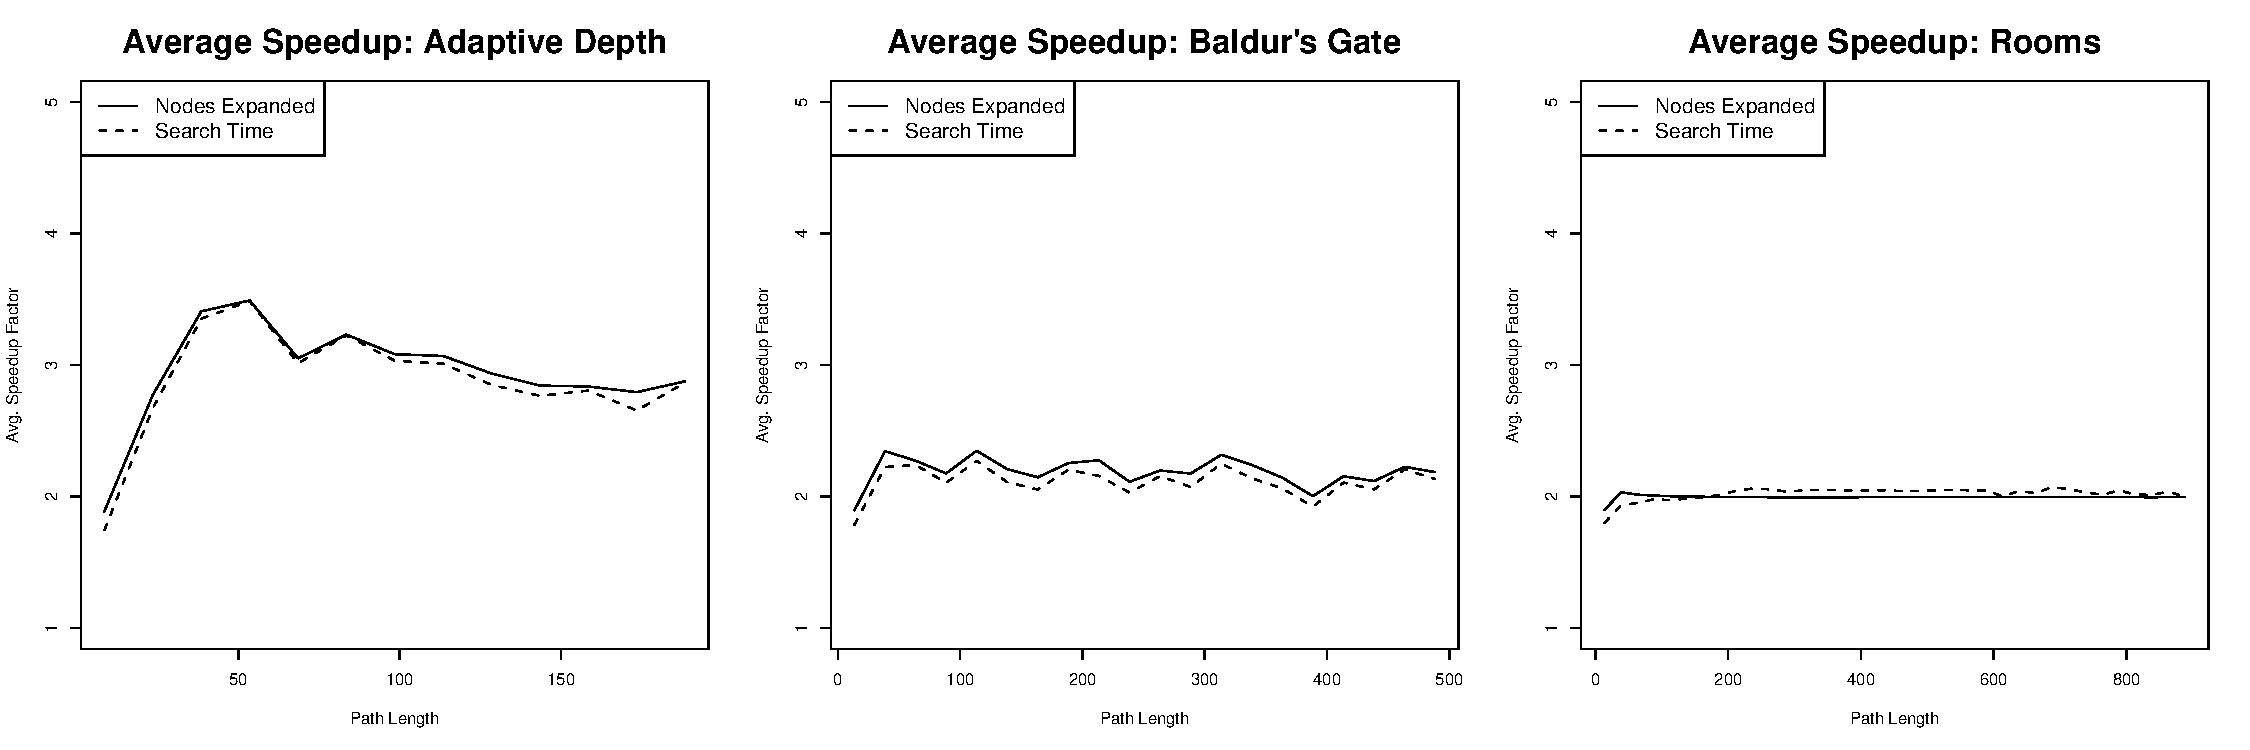
\includegraphics[width=1.95\columnwidth, trim = 10mm 10mm 10mm 0mm]{diagrams/speedup.pdf}
       \end{center}
       \caption{Average A* speedup on each of our three benchmarks. 
		Results are given in terms of nodes expanded and search time.}
\label{fig-speedup}
\end{figure*}
